\documentclass{classrep}
\usepackage[utf8]{inputenc}
\frenchspacing

\usepackage[usenames,dvipsnames]{color}
\usepackage[hidelinks]{hyperref}
\usepackage{float}
\usepackage{setspace}
\usepackage{amsmath, amssymb, mathtools}

\usepackage{graphicx}
\usepackage{booktabs}
\usepackage{pdflscape}

\setlength{\abovecaptionskip}{-10pt}

\studycycle{Informatyka stosowana, studia dzienne, II st.}
\coursesemester{II}
\coursename{Analiza danych złożonych}
\courseyear{2020/2021}

\courseteacher{dr hab. inż. Agnieszka Duraj}
\coursegroup{poniedziałek, 08:30}

\author{%
  \studentinfo{Paweł Galewicz}{234053}\\
  \studentinfo{Karol Podlewski}{234106}%
}

\title{Referat wykładowy -- Algorytm\\detekcji dryftu KSWIN}

\begin{document}
\maketitle

\setstretch{1.6}


KSWIN (Kolmogorov-Smirnov WINdowing) to algorytm służący do detekcji dryftu oparty na statystycznym teście Kołmogorowa-Smirnowa.

Test Kołmogorowa-Smirnowa jest testem nieparametrycznym, służącym do weryfikacji hipotezy o zgodności dwóch rozkładów empirycznych ze sobą. Może być stosowany między innymi do sprawdzenia zgodności rozkładu analizowanej zmiennej z rozkładem teoretycznym (na przykład normalnym, dwumianowym). Dobrze sprawdza się przy większych próbach badawczych - częstym proponowanym przedziałem jest N > 100. Istnieje też  wersja testu służąca do porównania rozkładów dwóch zmiennych losowych \cite{KST}.

Algorytm KSWIN, zaproponowany przez Raaba, Heusingera i Schleifa w \cite{KSWIN}, opiera się właśnie na teście Kołmogorowa-Smirnowa dla dwóch zmiennych. Potrzebuje on przesuwalnego okna $\Psi$ o stałym rozmiarze $n$, z którego tworzy dwa mniejsze okna na potrzeby przeprowadzenia testu. Pierwsze z nich posiada $r$ najnowszych punktów z okna $\Psi$:
\begin{equation}
R = \{x_i \ \epsilon \ \Psi\}^n_{i=n-r+1}
\end{equation}
Drugie okno jest tworzone poprzez jednolite próbkowanie z pozostałej części okna $n - r$:
\begin{equation}
W = \{x_i \  \epsilon \ \Psi | i < n - r + 1 \wedge p(x) = U(x_i|1,n-r) \}
\end{equation}
gdzie $U(x_i|1,n-r) = \frac{1}{n-r}$ jest rozkładem jednostajnym. 

Mając już dwie zmienne, możliwe jest przeprowadzenie testu Kołmogorowa-\\Smirnowa, który porównuje dystrybuanty empiryczne $F_W$ oraz $F_R$:
\begin{equation}
dist_{w,r} = \sup_{x} | F_W(x) - F_R(x)|
\end{equation}
gdzie $F_{(.)}(x)=\frac{1}{n}\sum^n_{j=1}I_{[-\infty,x]}(X_j)$ oraz $I_{[-\infty,x]}(X_j)$ to funkcja charakterystyczna, która przyjmuje wartość 1 jeżeli $X_i \geq x$ lub 0 w przeciwnym wypadku. $sup(x)$ to najmniejsza wartość, dla której warunek jest prawidłowy. Jeżeli kres górny jest większy od statystyki testowej, to hipoteza zerowa jest odrzucona, z poziomem istotności $\alpha$. Dryft jest znaleziony, kiedy hipoteza zerowa zostaje odrzucona - punkt wykrycia dryftu ustawiany jest na $n-r$. Następnie okno redukowane jest do ostatnich $r$ próbek.

Ze względu na czułość parametru $\alpha$ nie powinien być on większy niż 0,01 - będzie to skutkować zbyt częstym wykrywaniem dryftu. 

\begin{figure}[H]
    \centering
    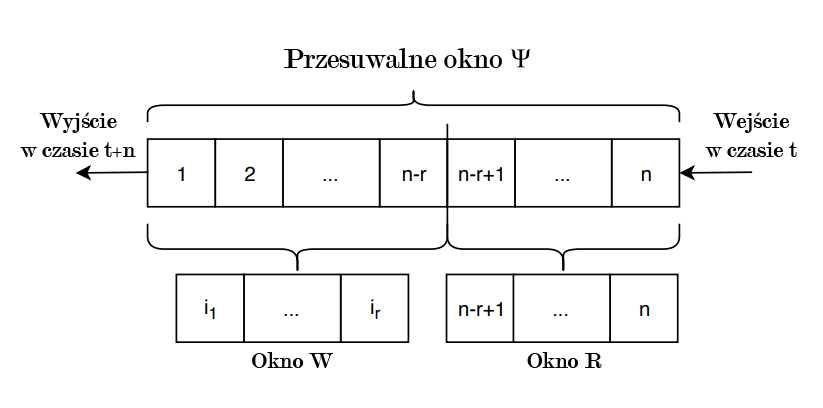
\includegraphics[width=1\textwidth]{resources/kswin/okno.png}
    \caption{Graficzna demonstracja podziału przesuwalnego okna $\Psi$}
    \label{DDM}
\end{figure}

Dla okien $W$ i $R$, które mają identyczny rozmiar, można zredukować test do postaci
\begin{equation}
dist_{w,r} > c(\alpha) \sqrt{\frac{w+r}{wr}} = \sqrt{-\frac{1}{2}\ln{\alpha}} \sqrt{\frac{w+r}{wr}} \overset{(w=r)}{=} \sqrt{-\frac{\ln{\alpha}}{r}},
\end{equation}
gdzie $\alpha$ to poziom istotności testu, $r$ oraz $w$ to rozmiary okien $R$ oraz $W$.$c(\alpha)$ to krytyczna wartość testu, która może zostać dostosowana do standardowych rozmiarów testu lub przyjęta jako $\sqrt{-\frac{1}{2}\ln{\alpha}}$. 

\newpage
\nocite{*}
\begin{thebibliography}{}

    \bibitem{KST}
    \textsl{SPSS Kolmogorov-Smirnov Test for Normality, }
    \author{Ruben Geert van den Berg. }
    \url{ https://www.spss-tutorials.com/spss-kolmogorov-smirnov-test-for-normality/}
    \text{ [dostęp: 04.01.2021]}

    \bibitem{KSWIN}
    \textsl{Reactive Soft Prototype Computing for Concept Drift Streams, }
    \author{Christoph Raab, Moritz Heusinger, Frank-Michael Schleif. }
    \url{ https://www.sciencedirect.com/science/article/abs/pii/S0925231220305063?via\%3Dihub}
    \text{ [dostęp: 04.01.2021]}

\end{thebibliography}

\end{document}
